\section{Figure}

\subsection{Subfigures}
Subfigure is a common techniques for showing images. In {\LaTeX}, there are several different packages for subfigures. Here we use the package \verb|subcaption| for an example, which is shown in Figure~\ref{Figure-Subfigures}.
\begin{figure}
    \centering
    \begin{subfigure}{0.3\linewidth}
        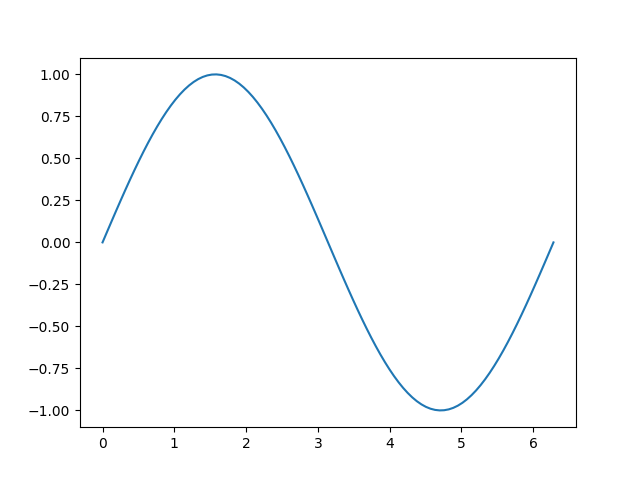
\includegraphics[width=\linewidth]{../figures/sin.png}
        \caption{\(y=\sin x, x\in[0,2\pi]\)}
    \end{subfigure}
    \begin{subfigure}{0.3\linewidth}
        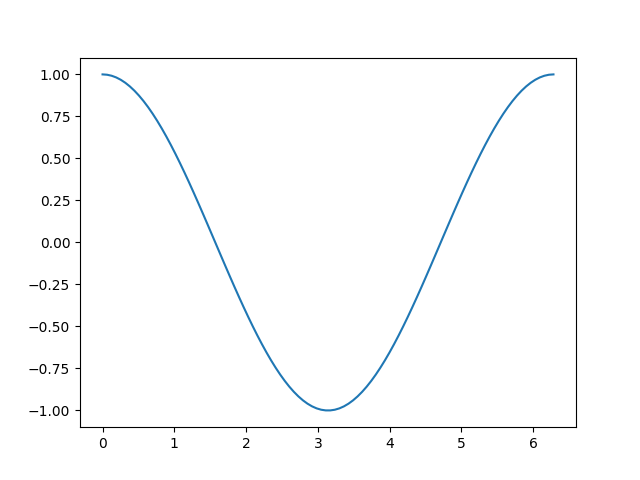
\includegraphics[width=\linewidth]{../figures/cos.png}
        \caption{\(y=\cos x, x\in[0,2\pi]\)}
    \end{subfigure}
    \\
    \begin{subfigure}{0.3\linewidth}
        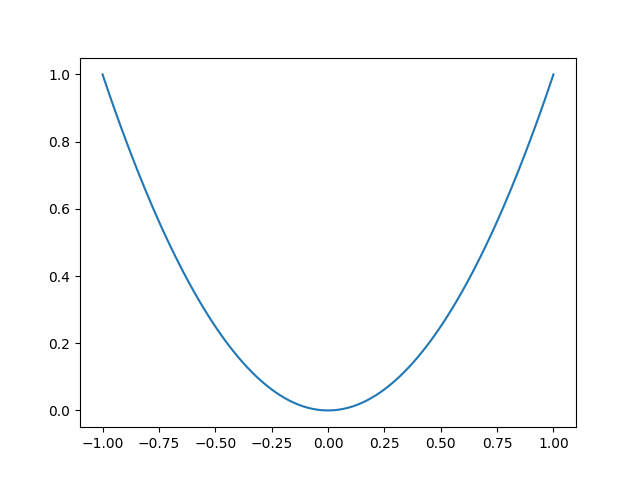
\includegraphics[width=\linewidth]{../figures/square.png}
        \caption{\(y=x^2, x\in[-1,1]\)}
    \end{subfigure}
    \begin{subfigure}{0.3\linewidth}
        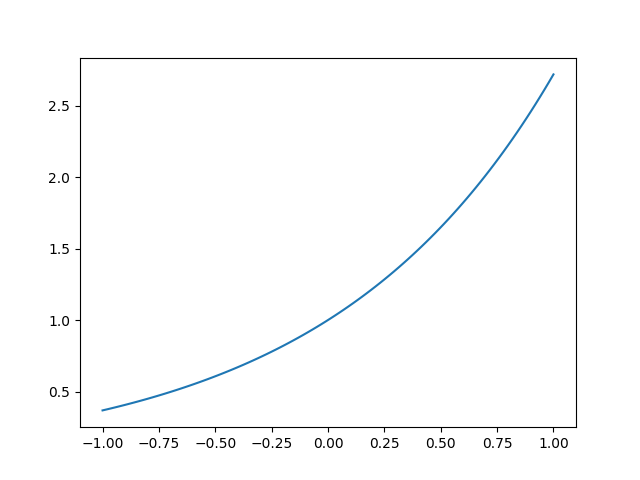
\includegraphics[width=\linewidth]{../figures/exp.png}
        \caption{\(y=\mathrm{e}^x, x\in[-1,1]\)}
    \end{subfigure}
    \caption{\textbf{Figure~\ref{Figure-Subfigures}.} Illustration of subfigures.}\label{Figure-Subfigures}
\end{figure}

\subsection{Vertical and Horizontal Label}
Sometimes we need to write row name and column name for subfigures grid. It is possible with command \verb|rotatebox|, \verb|phantom| and \verb|hspace|, but it's also very complicated. The effect is shown in
\begin{figure}
    \centering
    \rotatebox[origin=c]{90}{\phantom{1}}
    \hspace{0.02\linewidth}
    \begin{subfigure}{0.3\linewidth}
        \caption*{Col 1}
    \end{subfigure}
    \hspace{0.02\linewidth}
    \begin{subfigure}{0.3\linewidth}
        \caption*{Col 2}
    \end{subfigure}
    \\
    \rotatebox[origin=c]{90}{Row 1}
    \hspace{0.02\linewidth}
    \begin{subfigure}{0.3\linewidth}
        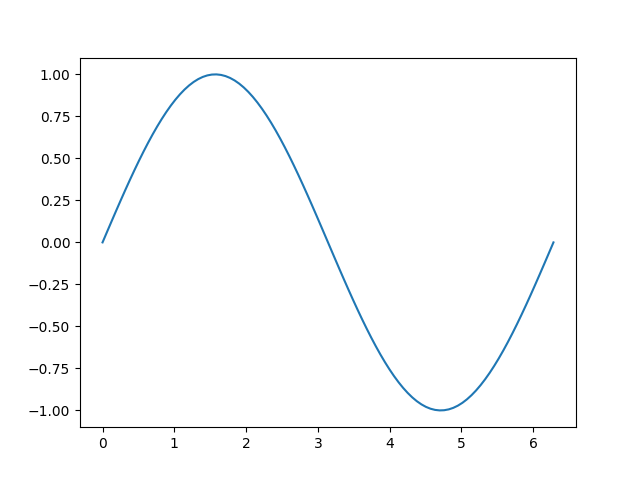
\includegraphics[width=\linewidth]{../figures/sin.png}
        \caption{\(y=\sin x, x\in[0,2\pi]\)}
    \end{subfigure}
    \hspace{0.02\linewidth}
    \begin{subfigure}{0.3\linewidth}
        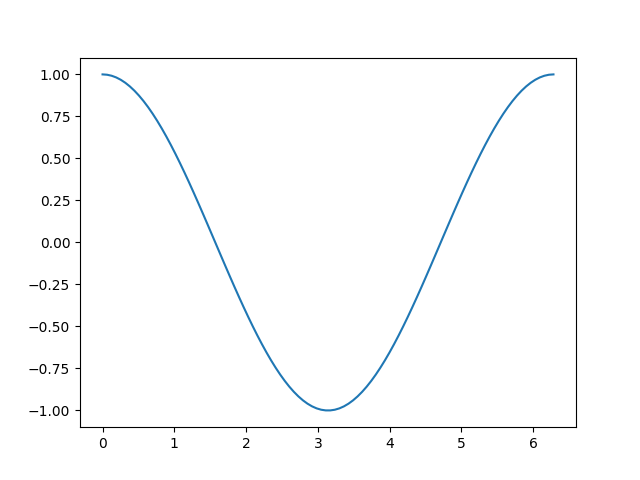
\includegraphics[width=\linewidth]{../figures/cos.png}
        \caption{\(y=\cos x, x\in[0,2\pi]\)}
    \end{subfigure}
    \\
    \rotatebox[origin=c]{90}{Row 2}
    \hspace{0.02\linewidth}
    \begin{subfigure}{0.3\linewidth}
        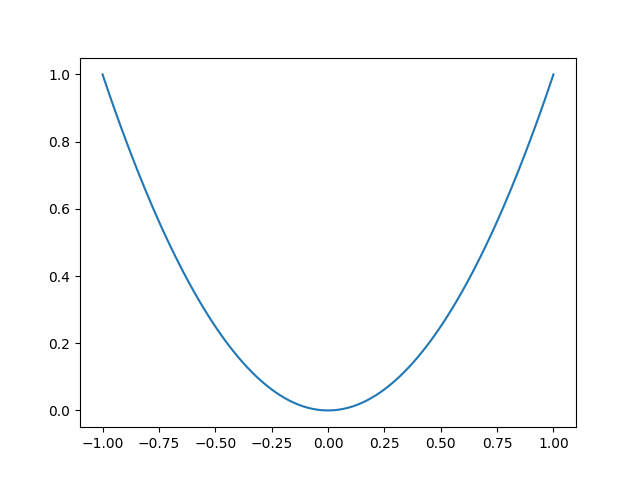
\includegraphics[width=\linewidth]{../figures/square.png}
        \caption{\(y=x^2, x\in[-1,1]\)}
    \end{subfigure}
    \hspace{0.02\linewidth}
    \begin{subfigure}{0.3\linewidth}
        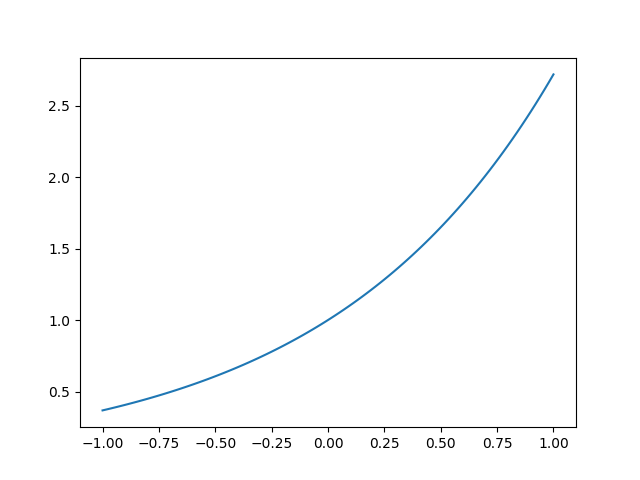
\includegraphics[width=\linewidth]{../figures/exp.png}
        \caption{\(y=\mathrm{e}^x, x\in[-1,1]\)}
    \end{subfigure}
    \caption{\textbf{Figure~\ref{Figure-VHLabels}.} Illustration of vertical and horizontal labels.}\label{Figure-VHLabels}
\end{figure}

\subsection{Combination of Figures and Tables}
We can insert tabular in a subfigure, so that figures and tables can be combined in a single image, which is shown in Figure~\ref{Figure-Mixed}.
\begin{figure}
    \centering
    \begin{subfigure}{0.3\linewidth}
        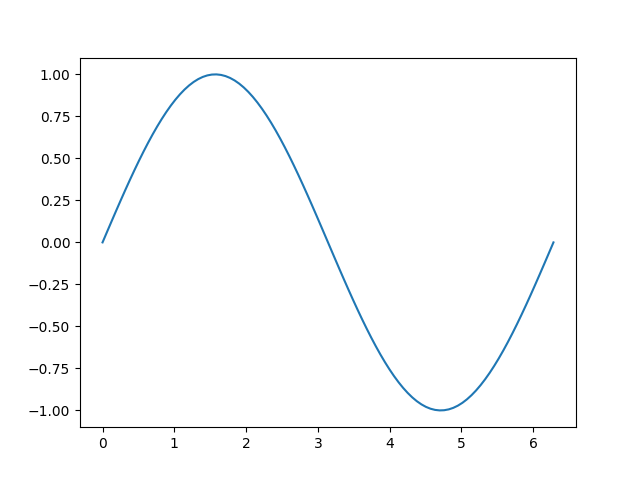
\includegraphics[width=\linewidth]{../figures/sin.png}
        \caption{\(y=\sin x, x\in[0,2\pi]\)}
    \end{subfigure}
    \begin{subfigure}{0.3\linewidth}
        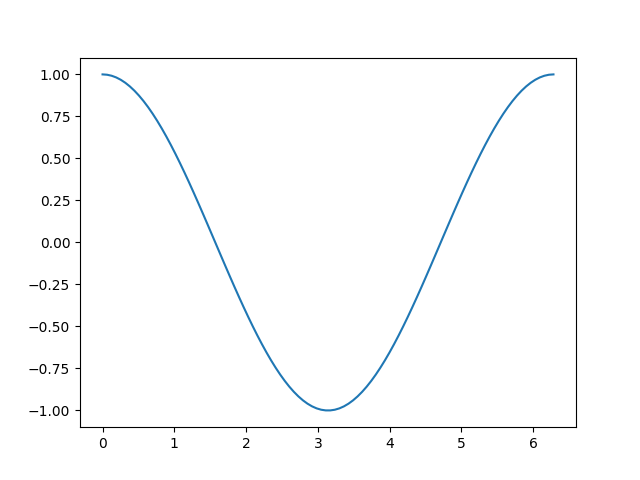
\includegraphics[width=\linewidth]{../figures/cos.png}
        \caption{\(y=\cos x, x\in[0,2\pi]\)}
    \end{subfigure}
    \\
    \begin{subfigure}{0.3\linewidth}
        \centering
        \begin{tabular}{ccccc}
            \toprule
            name & x & y & z & w \\
            \midrule
            a    & 1 & 2 & 3 & 4 \\
            b    & 1 & 2 & 3 & 4 \\
            c    & 1 & 2 & 3 & 4 \\
            \bottomrule
        \end{tabular}
        \caption{First Table}
    \end{subfigure}
    \begin{subfigure}{0.3\linewidth}
        \centering
        \begin{tabular}{ccccc}
            \toprule
            name                    & x & y & z & w \\
            \midrule
            \multirow{3}*{merged a} & 1 & 2 & 3 & 4 \\
            ~                       & 1 & 2 & 3 & 4 \\
            ~                       & 1 & 2 & 3 & 4 \\
            \bottomrule
        \end{tabular}
        \caption{Second Table}\label{Table-Merge-Lines}
    \end{subfigure}
    \caption{\textbf{Figure~\ref{Figure-Mixed}.} Illustration of figures and tables combination.}\label{Figure-Mixed}
\end{figure}
In Figure~\ref{Table-Merge-Lines}, we merged several lines of the row names. This can be used for merging cells. Package \verb|multirow| is required for such operation.
